%%==========================================================================
%%  Paper IEEE Conference  -  Visión por Computadora II (CEIA / FIUBA)
%%  Clasificación de régimen de mercado vía representaciones tiempo-frecuencia
%%  Compilar con pdflatex (2 pasadas) -> main.pdf
%%==========================================================================
\documentclass[conference]{IEEEtran}
\IEEEoverridecommandlockouts

\usepackage{cite}
\usepackage{amsmath,amssymb,amsfonts}
\usepackage{graphicx}
\usepackage{booktabs}
\usepackage{textcomp}
\usepackage{xcolor}
\usepackage[utf8]{inputenc}
\usepackage[T1]{fontenc}
\usepackage[spanish]{babel}
\usepackage{hyperref}

\begin{document}

\title{Clasificación de régimen de mercado mediante\\
representaciones tiempo--frecuencia y redes convolucionales}

\author{
\IEEEauthorblockN{Sofía Belén Caselli \quad Gaspar Rivollier \quad Miguel Ángel Leiva Martínez}
\IEEEauthorblockA{\textit{Especialización en Inteligencia Artificial} \\
\textit{Universidad de Buenos Aires (FIUBA)} ---
Buenos Aires, Argentina}
}

\maketitle

%%--------------------------------------------------------------------------
\begin{abstract}
Se aborda la predicción de señales de \emph{trading} (comprar, mantener,
vender) transformando la serie temporal de precios en imágenes
tiempo--frecuencia y procesándolas con redes neuronales convolucionales
(CNN). Sobre un universo multi--activo (criptomonedas, acciones, materias
primas y divisas) se generan dos representaciones de cada ventana de 60
días: el espectrograma de Fourier de tiempo corto (STFT) y el escalograma
\emph{wavelet} de Morlet continua. Las etiquetas se construyen con un umbral
adaptativo basado en el \emph{Average True Range} (ATR) y se reserva el año
2026 como conjunto de prueba estrictamente fuera de muestra. Se comparan
cuatro modelos bajo idénticas condiciones (CNN propia y ResNet--18
preentrenada, cada una con STFT y \emph{wavelet}), evaluados con
\emph{balanced accuracy} y F1--macro para evitar el sesgo del desbalance de
clases. La mejor combinación, ResNet--18 sobre STFT, alcanza un F1--macro de
0,369 y \emph{balanced accuracy} de 37,4\,\%,
superando el azar (0,333) y al resto de las configuraciones. Los resultados
muestran que (i) el \emph{transfer learning} domina a la CNN entrenada desde
cero y (ii) la STFT captura mejor la señal direccional que el escalograma
\emph{wavelet} en esta tarea. La señal predictiva existe pero es débil, lo
que constituye un hallazgo honesto sobre los límites del enfoque puramente
visual en mercados financieros.
\end{abstract}

\begin{IEEEkeywords}
series temporales financieras, STFT, transformada wavelet continua, redes
convolucionales, transfer learning, clasificación de régimen de mercado.
\end{IEEEkeywords}

%%--------------------------------------------------------------------------
\section{Introducción}

La predicción de la dirección de los mercados financieros es un problema
clásico por su relevancia económica y su dificultad: las series de precios
son no estacionarias, ruidosas y con baja relación señal--ruido. Una línea
de trabajo creciente propone \emph{re--encuadrar} el problema como uno de
visión por computadora, convirtiendo la serie en una imagen y delegando la
extracción de patrones a una CNN, en analogía con el análisis gráfico
("técnico") tradicional.

Este trabajo explora esa hipótesis con representaciones \emph{tiempo--
frecuencia}, que exponen explícitamente cómo evoluciona el contenido
frecuencial del precio a lo largo del tiempo. La motivación productiva es
generar señales de \emph{trading} accionables (BUY/HOLD/SELL) a partir de
patrones visuales en la dinámica de frecuencias.

A diferencia de una representación puramente temporal, un mapa
tiempo--frecuencia hace explícita la coexistencia de ciclos de distinta
duración: tendencias de mediano plazo (bajas frecuencias) y oscilaciones
rápidas o \emph{shocks} (altas frecuencias). La hipótesis de trabajo es que
los regímenes de mercado --- alcista, lateral, bajista --- dejan una
\emph{firma} reconocible en este plano, y que una CNN, sin ingeniería de
\emph{features} manual, puede aprender a discriminarla. La elección de
\emph{qué} representación tiempo--frecuencia usar (Fourier vs.\ \emph{wavelet})
no es neutral: cada una impone un compromiso distinto entre resolución
temporal y frecuencial, lo que motiva el \emph{ablation} central de este
estudio.

\subsection{Estado del arte}

El uso de CNN sobre imágenes de mercado fue popularizado por Sezer y Ozbayoglu
\cite{sezer2018}, quienes codifican indicadores técnicos en una grilla 2D
(\emph{CNN--TA}) y entrenan una CNN para emitir señales de compra/venta,
obteniendo resultados competitivos frente a estrategias \emph{buy-and-hold}.
Más recientemente, Cohen \emph{et al.} \cite{cohen2020} y diversos trabajos
sobre \emph{Gramian Angular Fields} \cite{wang2015} confirman que la
transformación serie--a--imagen permite reutilizar arquitecturas de visión
preentrenadas. En el dominio tiempo--frecuencia, el escalograma
\emph{wavelet} ha mostrado ventajas para detectar eventos transitorios
(\emph{crashes}, picos) gracias a su resolución adaptativa
\cite{torrence1998}. Nuestra contribución es un \emph{ablation} controlado
que enfrenta STFT contra \emph{wavelet} de Morlet bajo idénticas condiciones
de entrenamiento y evaluación, sobre un universo multi--activo y con un
protocolo temporal estricto (test = 2026).

\subsection{Contribuciones}
\begin{itemize}
  \item Un \emph{pipeline} reproducible que genera, para cada activo, dos
        datasets de imágenes (STFT y \emph{wavelet}) con etiquetas idénticas.
  \item Un etiquetado BUY/HOLD/SELL con umbral adaptativo por ATR escalado
        con la raíz del horizonte temporal.
  \item Una comparación de cuatro modelos y un barrido de horizontes,
        reportando métricas robustas al desbalance de clases.
\end{itemize}

%%--------------------------------------------------------------------------
\section{Metodología}

\subsection{Datos y preprocesamiento}
Se descargan precios diarios ajustados vía \texttt{yfinance} desde
2022-01-01. El universo cubre cuatro clases de activo: criptomonedas,
acciones, materias primas y divisas. Para cada activo se calcula la serie de
retornos logarítmicos $r_t = \log(P_t / P_{t-1})$, estacionaria y aditiva,
y se la normaliza por \emph{z-score}. Cada muestra es una ventana deslizante
de $W=60$ días.

\subsection{Representaciones tiempo--frecuencia}
A partir de cada ventana se generan dos imágenes de $64\times64$ píxeles
(mapa de color \emph{magma}, frecuencias bajas abajo):
\begin{itemize}
  \item \textbf{STFT}: espectrograma con ventana de Hann de 32 muestras,
        solapamiento de 28 y \texttt{nfft}=64. Resolución
        tiempo--frecuencia fija.
  \item \textbf{Wavelet}: transformada \emph{wavelet} continua con Morlet
        compleja \texttt{cmor1.5-1.0} y escalas de 2 a 30 días. Resolución
        adaptativa, mejor para transitorios.
\end{itemize}
Ambos datasets comparten exactamente las mismas etiquetas, lo que permite un
\emph{ablation} limpio de la representación. La Fig.~\ref{fig:repr} ilustra
ambas transformaciones sobre una misma ventana de precio: la STFT ofrece una
grilla tiempo--frecuencia de resolución uniforme, mientras que el escalograma
\emph{wavelet} concentra mayor detalle en los eventos transitorios (la caída
del precio se refleja en la activación de las escalas correspondientes).

\begin{figure*}[t]
\centering
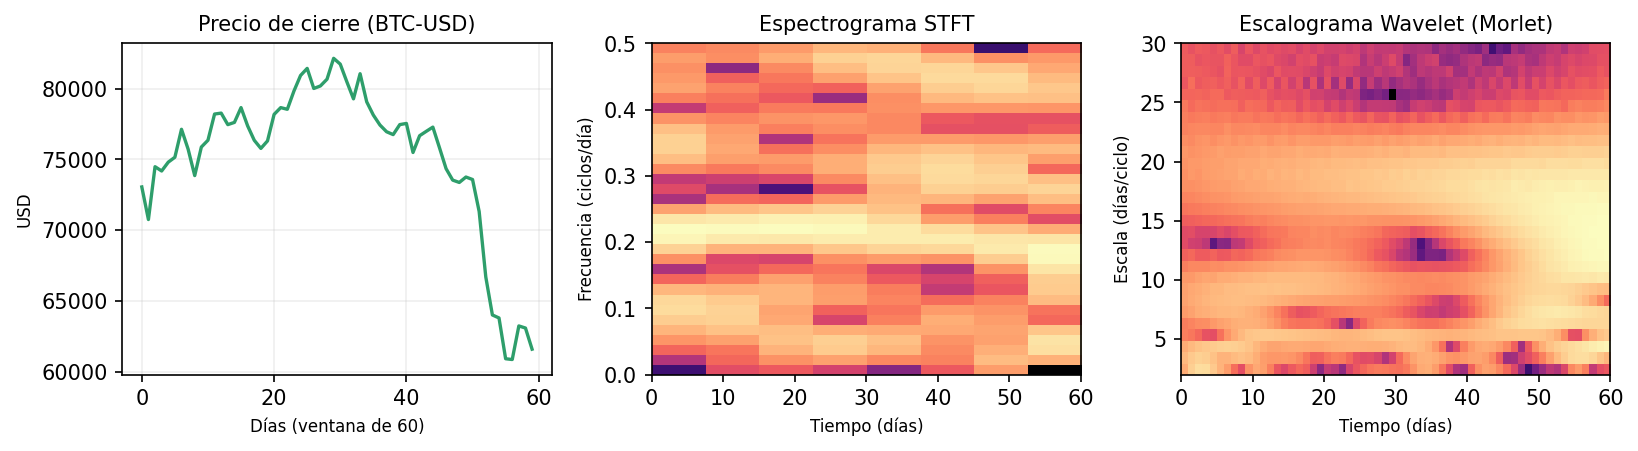
\includegraphics[width=\textwidth]{figs/representaciones.png}
\caption{De serie de precios a imagen tiempo--frecuencia. Izquierda: ventana
de 60 días del precio de cierre. Centro: espectrograma STFT (resolución
fija). Derecha: escalograma \emph{wavelet} de Morlet (resolución adaptativa).
Ambas se redimensionan a $64\times64$ con mapa \emph{magma} como entrada a la
CNN.}
\label{fig:repr}
\end{figure*}

\subsection{Etiquetado adaptativo}
La etiqueta de cada muestra depende del retorno futuro acumulado a $h$ días y
de un umbral proporcional a la volatilidad local, medida con el ATR:
\begin{equation}
\text{label}=
\begin{cases}
\text{BUY}  & \text{si } R_h > +\tau_h\\
\text{SELL} & \text{si } R_h < -\tau_h\\
\text{HOLD} & \text{en otro caso}
\end{cases}
\end{equation}
con $\tau_h = k \cdot \mathrm{ATR} \cdot \sqrt{h}$ y $k=0{,}7$. El factor
$\sqrt{h}$ refleja que la volatilidad crece con la raíz del tiempo. El umbral
$k$ se ajustó para mitigar el dominio de la clase HOLD. Un valor inicial de
$k=1{,}3$ producía una distribución degenerada ($\sim$90\,\% HOLD) que
inducía el colapso del clasificador a la clase mayoritaria; reducirlo a
$k=0{,}7$ equilibró la distribución a aproximadamente
17\,\%/68\,\%/15\,\% (BUY/HOLD/SELL), sin dejar de respetar la semántica de
volatilidad del ATR. Este ajuste ilustra cómo el diseño del etiquetado, y no
sólo el modelo, condiciona fuertemente el aprendizaje en problemas
financieros.

\subsection{Protocolo de evaluación}
El \emph{split} es estrictamente cronológico para evitar fuga temporal:
entrenamiento y validación dentro de 2022--2025 (validación = últimos meses),
y \textbf{2026 completo como test fuera de muestra}. El conjunto resultante
tiene aproximadamente 6.700 muestras (train 4.690, val 1.496, test 523 para
el horizonte de 7 días).

\subsection{Modelos y entrenamiento}
Se comparan dos arquitecturas:
\begin{itemize}
  \item \textbf{CNN propia}: cuatro bloques convolucionales
        (Conv--BN--ReLU$\times2$--MaxPool--Dropout), $\sim$1,45\,M de
        parámetros, entrenada desde cero.
  \item \textbf{ResNet--18}: backbone preentrenado en ImageNet
        (\emph{transfer learning}) con cabeza densa de tres clases,
        $\sim$11,24\,M de parámetros.
\end{itemize}
El desbalance de clases se ataca con doble mecanismo: \emph{Weighted Random
Sampler} y \emph{Cross Entropy} ponderada por el inverso de la frecuencia,
con \emph{label smoothing} 0,05. Optimizador AdamW
($\text{lr}=3\times10^{-4}$, \emph{weight decay} $10^{-4}$),
\emph{ReduceLROnPlateau}, \emph{early stopping} sobre F1--macro de
validación y \emph{gradient clipping}. Todos los experimentos comparten
semilla, épocas, transformaciones y \emph{split}, garantizando
\emph{idénticas condiciones}.

%%--------------------------------------------------------------------------
\section{Resultados}

\subsection{Comparación de modelos}
La Tabla~\ref{tab:comp} resume las cuatro combinaciones sobre el test 2026,
ordenadas por F1--macro. Dado el fuerte desbalance (HOLD $\approx$ 68\,\%),
la \emph{accuracy} cruda es engañosa; las métricas principales son
\emph{balanced accuracy} y F1--macro.

\begin{table}[t]
\caption{Comparación de modelos (test 2026, horizonte 7 días).}
\label{tab:comp}
\centering
\begin{tabular}{llcccr}
\toprule
\textbf{Modelo} & \textbf{Repr.} & \textbf{Acc \%} & \textbf{Bal-Acc \%} & \textbf{F1-macro} & \textbf{Params} \\
\midrule
ResNet--18 & STFT    & 62,33 & 37,43 & \textbf{0,369} & 11,24\,M \\
ResNet--18 & Wavelet & 51,24 & 30,42 & 0,305 & 11,24\,M \\
CNN propia & STFT    & 25,24 & 36,42 & 0,243 & 1,45\,M \\
CNN propia & Wavelet & 16,63 & 38,00 & 0,167 & 1,45\,M \\
\midrule
\multicolumn{2}{l}{\textit{Azar (3 clases)}} & 33,3 & 33,3 & 0,333 & --- \\
\bottomrule
\end{tabular}
\end{table}

\begin{figure}[t]
\centering
% Copiar resultados/comparacion_modelos.png a paper/figs/ antes de compilar
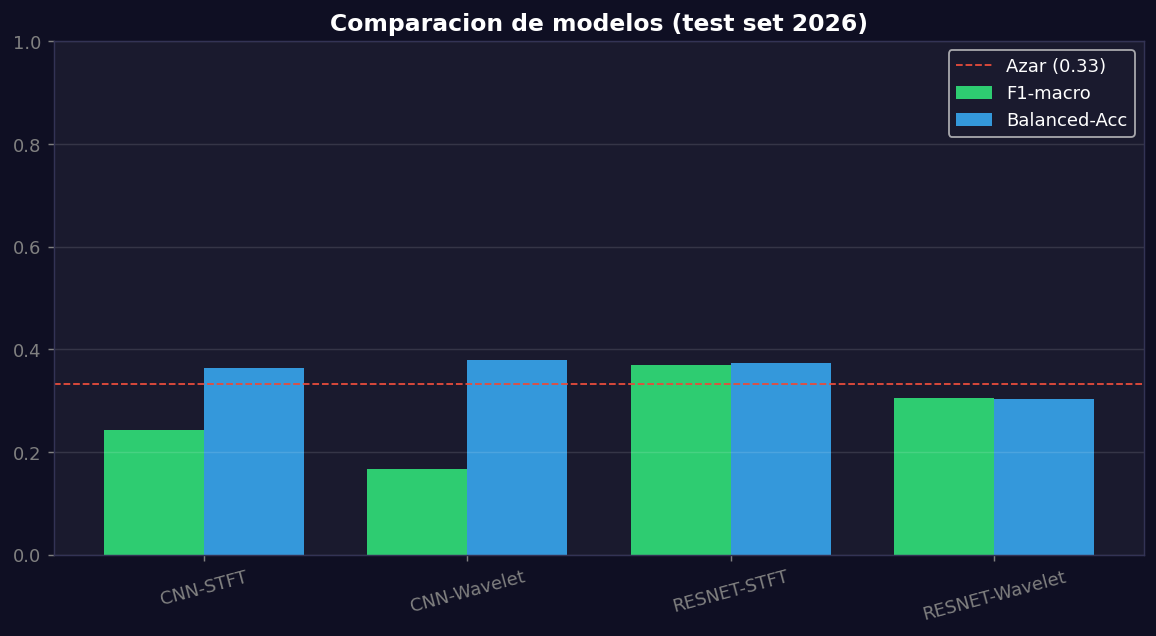
\includegraphics[width=\columnwidth]{figs/comparacion_modelos.png}
\caption{F1--macro y \emph{balanced accuracy} por modelo. La línea punteada
marca el azar (0,33).}
\label{fig:comp}
\end{figure}

\subsection{Ablation de representación}
En ambas arquitecturas la STFT supera al escalograma \emph{wavelet}
(ResNet: 0,369 vs.\ 0,305; CNN: 0,243 vs.\ 0,167). Pese a la mejor
resolución del \emph{wavelet} para transitorios, la STFT aporta mayor señal
direccional global en esta tarea.

\subsection{Barrido de horizontes}
Sobre el modelo ganador (ResNet--STFT) se evaluaron tres horizontes
(Tabla~\ref{tab:hor}). El horizonte corto (7 días) maximiza el F1--macro;
ampliar el horizonte degrada levemente el desempeño.

\begin{table}[t]
\caption{Barrido de horizontes (ResNet--STFT, test 2026).}
\label{tab:hor}
\centering
\begin{tabular}{cccc}
\toprule
\textbf{Horizonte (d)} & \textbf{Acc \%} & \textbf{Bal-Acc \%} & \textbf{F1-macro} \\
\midrule
7  & 62,33 & 37,43 & \textbf{0,369} \\
15 & 51,63 & 35,62 & 0,342 \\
30 & 61,95 & 35,05 & 0,338 \\
\bottomrule
\end{tabular}
\end{table}

\begin{figure}[t]
\centering
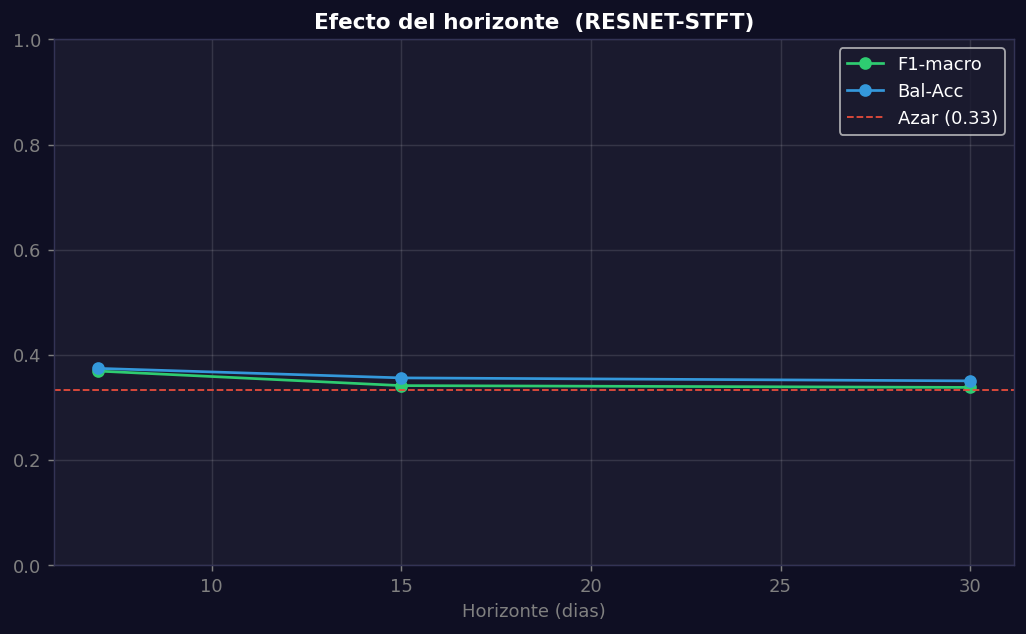
\includegraphics[width=\columnwidth]{figs/barrido_horizontes.png}
\caption{Desempeño de ResNet--STFT según el horizonte de predicción. El
horizonte de 7 días maximiza el F1--macro y la \emph{balanced accuracy}.}
\label{fig:hor}
\end{figure}

\subsection{Análisis por clase}
La Tabla~\ref{tab:report} detalla el reporte de clasificación del mejor
modelo (ResNet--STFT, 7 días) sobre el test 2026. El modelo identifica bien
la clase mayoritaria HOLD (\emph{recall} 0,81) pero tiene dificultad con las
señales accionables BUY (\emph{recall} 0,26) y especialmente SELL
(\emph{recall} 0,06). Esto indica que la mayor parte de la ganancia sobre el
azar proviene de detectar la \emph{ausencia} de señal direccional fuerte más
que de anticipar el sentido del movimiento.

\begin{table}[t]
\caption{Reporte por clase --- ResNet--STFT, horizonte 7 días, test 2026.}
\label{tab:report}
\centering
\begin{tabular}{lcccc}
\toprule
\textbf{Clase} & \textbf{Precision} & \textbf{Recall} & \textbf{F1} & \textbf{Soporte} \\
\midrule
BUY  & 0,282 & 0,256 & 0,268 & 78 \\
HOLD & 0,721 & 0,812 & 0,764 & 372 \\
SELL & 0,121 & 0,055 & 0,075 & 73 \\
\midrule
\textit{macro avg}    & 0,375 & 0,374 & 0,369 & 523 \\
\textit{weighted avg} & 0,572 & 0,623 & 0,594 & 523 \\
\bottomrule
\end{tabular}
\end{table}

\subsection{Interpretabilidad}
Se aplicó Grad--CAM sobre la última capa convolucional del modelo ganador
para identificar qué regiones del espectrograma motivan cada decisión. Las
activaciones se concentran predominantemente en las bandas de \emph{baja
frecuencia} (parte inferior de la imagen, ciclos largos), lo que es
consistente con el predominio de la componente tendencial del precio por
sobre el ruido de alta frecuencia. Este comportamiento sugiere que la red
aprende a leer la inercia de mediano plazo de la serie más que oscilaciones
rápidas, alineado con la intuición del análisis técnico tradicional.

\subsection{Costo computacional}
La CNN propia (1,45\,M de parámetros) es casi un orden de magnitud más
liviana que ResNet--18 (11,24\,M), pero su menor capacidad y la falta de
preentrenamiento la dejan por debajo en todas las métricas. El compromiso
costo--desempeño favorece claramente al \emph{transfer learning} en este
problema: el sobrecosto de ResNet se traduce en una mejora de F1--macro de
$+0{,}126$ con STFT.

%%--------------------------------------------------------------------------
\section{Discusión y limitaciones}

Los resultados deben leerse con cautela. En primer lugar, la métrica
\emph{accuracy} resulta profundamente engañosa bajo el desbalance observado:
un clasificador trivial que prediga siempre HOLD obtendría $\sim$68\,\% de
\emph{accuracy} y, sin embargo, sería inútil como sistema de \emph{trading}.
Por ello todo el análisis se ancla en \emph{balanced accuracy} y F1--macro,
que penalizan explícitamente ignorar a las clases minoritarias.

En segundo lugar, la superioridad de la STFT sobre el escalograma
\emph{wavelet} puede deberse en parte a la dimensión y el preprocesamiento
de las imágenes ($64\times64$, reescaladas): a esa resolución, la ventaja de
localización del \emph{wavelet} para transitorios podría diluirse. No puede
descartarse que con mayor resolución, o combinando ambas representaciones en
canales separados, el balance cambie.

En tercer lugar, el conjunto de prueba (2026) corresponde a un único año y a
un régimen de mercado particular; la generalización temporal a otros
períodos no está garantizada. Asimismo, la evaluación es puramente de
clasificación y no incorpora costos de transacción ni un \emph{backtesting}
económico, por lo que un F1--macro superior al azar no implica
automáticamente rentabilidad.

Finalmente, la dificultad para predecir BUY y SELL es coherente con la
hipótesis de eficiencia de mercado: si la dirección futura fuese fácilmente
legible en el espectrograma, la oportunidad de arbitraje se cerraría
rápidamente. El valor del trabajo radica, entonces, no en una promesa de
rentabilidad sino en cuantificar de forma controlada \emph{cuánta} señal
direccional es extraíble por métodos visuales, y en establecer un protocolo
reproducible para futuras mejoras.

%%--------------------------------------------------------------------------
\section{Conclusiones}
\begin{enumerate}
  \item \textbf{El \emph{transfer learning} es decisivo}: ResNet--18
        preentrenada supera ampliamente a la CNN entrenada desde cero
        (F1--macro 0,369 vs.\ 0,243 con STFT), pese a la diferencia de
        dominio entre ImageNet y los espectrogramas financieros.
  \item \textbf{STFT $>$ Wavelet en esta tarea}: la representación de Fourier
        captura mejor la señal direccional global, superando al escalograma
        de Morlet en ambas arquitecturas.
  \item \textbf{Horizonte corto preferible}: 7 días maximiza el F1--macro;
        horizontes mayores no mejoran y tienden a degradar.
  \item \textbf{La señal existe pero es débil}: la \emph{balanced accuracy}
        del 37,4\,\% supera el azar (33,3\,\%) de forma modesta; las clases
        BUY/SELL son difíciles de detectar, lo que delimita honestamente el
        alcance del enfoque visual.
  \item \textbf{La evaluación honesta es imprescindible}: una
        \emph{accuracy} cruda del 62\,\% oculta el colapso a la clase
        mayoritaria; sólo \emph{balanced accuracy} y F1--macro revelan el
        desempeño real, y deben ser el criterio en datasets desbalanceados.
\end{enumerate}

Como trabajo futuro se proponen: \emph{focal loss} para reforzar las clases
minoritarias, fusión de ambas representaciones en canales separados,
horizontes intradía y validación con \emph{backtesting} económico.

%%--------------------------------------------------------------------------
\begin{thebibliography}{00}
\bibitem{sezer2018} O.~B. Sezer and A.~M. Ozbayoglu, ``Algorithmic financial
trading with deep convolutional neural networks: Time series to image
conversion approach,'' \emph{Applied Soft Computing}, vol.~70,
pp.~525--538, 2018.

\bibitem{cohen2020} N.~Cohen, T.~Balch, and M.~Veloso, ``Trading via image
classification,'' in \emph{Proc. ACM Int. Conf. on AI in Finance (ICAIF)},
2020.

\bibitem{wang2015} Z.~Wang and T.~Oates, ``Imaging time-series to improve
classification and imputation,'' in \emph{Proc. IJCAI}, 2015,
pp.~3939--3945.

\bibitem{torrence1998} C.~Torrence and G.~P. Compo, ``A practical guide to
wavelet analysis,'' \emph{Bulletin of the American Meteorological Society},
vol.~79, no.~1, pp.~61--78, 1998.
\end{thebibliography}

\end{document}
